\chapter{Introduction}

\section{Formation de la synapse}
	\label{sec:IntroSynapse}
	La formation de synapses, ou synaptogenèse, consiste en un rapprochement d'un élément pré-synaptique, le cône de croissance de l'axone, et d'une élément post-synaptique, généralement les dendrites d'un neurones, mais pouvant également être un muscle dans le cas de \gls{jnm}. Bien que la synaptogenèse survient tout au long de la vie d'un individu, la majorité de celle-ci survient dans le \gls{snc} lors du développement précoce. On estime que dans un cerveau adulte se trouve environ 10\up{15}	synapses. Ces synapses sont des structures asymétriques, permettant généralement le passage d'un neurotransmetteurs de l'élément pré-synaptique pour aller activer un récepteur au niveau de l'élément post-synaptique. Les synapses sont donc des structures nécessaires au bon fonctionnement du cerveau. 
	
	La \gls{jnm} est une structure appartenant au \gls{snp}, et qui fait le lien entre le motoneurone et la fibre musculaire squelettique. De part sa grande taille et sa facilité d'accès, la \gls{jnm} est depuis longtemps le modèle préférentiel pour étudier les synapses. Chez les vertébrés, le neurotransmetteur utilisé à la \gls{jnm} est l'\gls{ach}. La mise en place de l'élément pré-synaptique requiert un alignement correct des agrégats de \glspl{achr} au milieu de la fibre musculaire, agrégats qui commencent à se former avant l'arrivée de l'axone \cite{Wu2010a, Gordon2012}. Cette étape qui se déroule avant la venue de l'axone se nomme "pré-patterning".
	
	Lors du développement, le cône de croissance de l'axone va se diriger vers l'élément post-synaptique. Quand les deux éléments entrent en contacts (après environ 2 semaines de gestation chez la souris), des cascades de signalisation sont initiés, ce qui résulte en la différentiation des partie pré- et post-synaptiques \cite{Sanes1999}, avec notamment une redistribution des clusters de \glspl{achr}, qui ne sont plus présent dans les région extrasynaptiques.
	
	\begin{wrapfigure}{L}{\textwidth}
		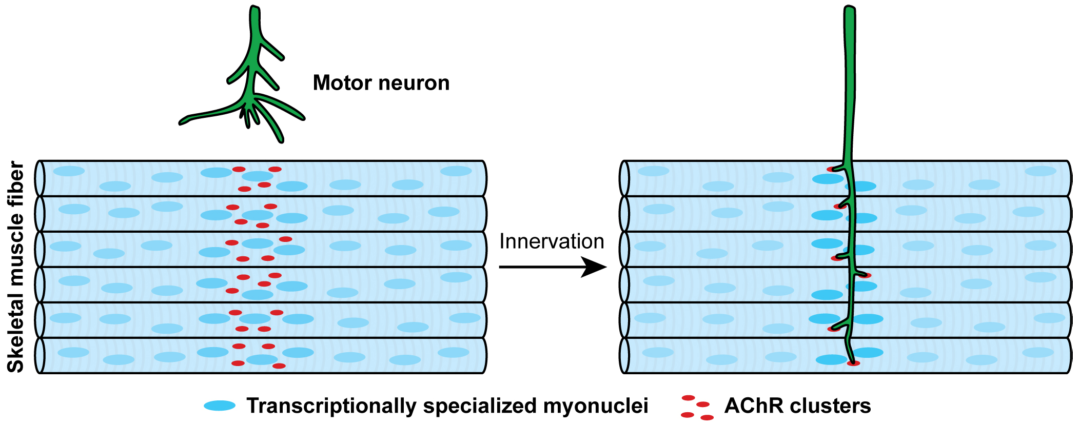
\includegraphics[width=\textwidth]{./Images/formation_jnm.png}
		
		\caption{Formation de la \gls{jnm}}
		\label{fig:FormaJNM}
	\end{wrapfigure}
	\clearpage
	
	Cette accumulation de \glspl{achr} est due à un récepteur particulier : \gls{musk}. Ce dernier joue un rôle clef dans la formation de la synapse, sa position déterminant la position de cette dernière \cite{DeChiara1996, Glass1996}. Le ligand activateur de \gls{musk} est historiquement l'Agrine \cite{Glass1996}, qui est sécrété par l'axone approchant. Plus récemment, des travaux ont montré que l'Agrine se fixait sur le co-récepteur de \gls{musk} : le récepteur \gls{lrp4} \cite{Zhang2008, Kim2008}. Suite à l'activation par l'Agrine de \gls{lrp4}, deux complexes \gls{musk}/\gls{lrp4} vont s'assembler, et l'assemblage tétramérique permettrait une meilleure phosphorylation de \gls{musk}, et donc une meilleure différenciation de la synapse et de l'agrégation des \gls{achr} \cite{Zong2012}.
	
\section{Récépteur MuSK}
	\label{sec:IntroMuSK}
	
	\begin{wrapfigure}{l}{0.1\textwidth}
		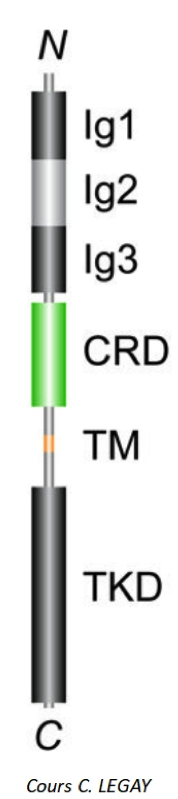
\includegraphics[width=0.1\textwidth]{./Images/MuSKReceptor.png}	
		\caption{Récepteur \gls{musk}}
		\label{fig:RMuSK}
	\end{wrapfigure}

	\gls{musk} est un récepteur découvert dans l'organe électrique d'anguille \emph{Torpedo california}. Ce récepteur a premièrement été connu pour être exprimé par les cellules musculaire au niveau de la \gls{jnm}. \gls{musk} est une récepteur tyrosine-kinase de 98kDa, divisé en trois parties : un ectodomaine (partie N-terminale), un domaine transmembranaire, et un domaine cytoplasmique qui porte l'activité kinasique (voir \Cref{fig:RMuSK}). 
	
	La partie extracellulaire comporte généralement trois domaines \gls{ig}, dont le domaine \gls{ig}1 a récemment été impliqué dans la liaison avec \gls{lrp4} \cite{Zhang2011}, ainsi qu'un domaine Frizzled-like, riche en cystéine (\gls{crd}). \gls{wnt}2, 3a, 4, 6, 7b, 9a, et 11 \cite{Stiegler2009}. 
	
	\gls{musk} possède trois ligand connu : l'Agrine (via \gls{lrp4}), l'\gls{colq} et les \gls{wnt}, tous nécessaire au bon développement de la synapse. Un défaut de signalisation de l'un d'entre eux entraîne ainsi des défauts moteurs importants.
	
	La présence de \gls{musk} dans le cerveau a longtemps été ignorée, à cause de techniques comme le Northern Blot, trop peu sensible. Cependant, de nouvelles techniques, telle que l'\gls{his} ou bien la \gls{qpcr}, ont permis de montrer que le récepteur se trouvait bien dans le tissu cérébral, bien qu'exprimé en faible quantité, principalement au niveau du cortex, du cervelet, et de l'hippocampe \cite{Garcia-Osta2006, Ksiazek2007}. On sait désormais, grâce à des techniques de Knockdown du gène, que la présence de \gls{musk} dans le cerveau est nécessaire à la formation de la mémoire, au travers de la voie \gls{creb} : l'absence de \gls{musk} va empêché la phosphorylation \gls{creb}. De plus, \gls{musk} est nécessaire à la formation de la \gls{ltp} de l'hippocampe \cite{Garcia-Osta2006}.
	
\section{Protéines \gls{wnt}}
	\label{sec:IntroWnt}
	
	Les protéines \gls{wnt} sont des glycoprotéines sécrétées, de 40kDa, et impliquées dans de nombreux processus développementaux tel que l'embryogenèse, la prolifération, la différenciation, la migration cellulaire, ou encore l'apoptose \cite{Miller2002, Willert2012a}. En plus de leur rôles durant le développement, les \glspl{wnt} jouent également un rôle à l'age adulte dans la maintenance des tissus adultes. Des travaux ont pu montrer que les \glspl{wnt} étaient également impliqués dans la formation de la \gls{jnm} \cite{Hall2000}. On connaît actuellement 19 membres de cette famille chez la souris et chez l'humain. Classiquement, les \Glspl{wnt} se lie sur le récepteur \gls{fz} avec les co-récepteur LRP5/6. Mais il existe d'autres récepteurs tels que : \gls{ror}, \gls{ryk}, ou bien encore \gls{musk}, grâce à son \gls{crd}.
	
	Il a été montré \emph{in vitro} que plusieurs \glspl{wnt} interagissaient avec \gls{musk} : \gls{wnt}2, 3a, 4, 6, 7b, 9a, et 11 \cite{Strochlic2012, Zhang2012, Barik2014}, avec différents effets. Seules \gls{wnt}4, 9a et 11 vont conduire à une dimérisation de \gls{musk} et a son activation (\emph{in vitro}). Ceci est cohérent avec le fait que chez le Poisson-zèbre, l'orthologue de \gls{musk}, \emph{unplugged}, le \gls{crd} allait interagir avec des protéines \gls{wnt} pour induire l'agrégation de \gls{achr} \cite{Jing2009, Gordon2012}. De plus, \gls{lrp4} semble être également nécessaire à l'agrégation des \gls{achr} médié par les \gls{wnt}s \cite{Zhang2012}.
	
	Les protéines \gls{wnt} vont activer plusieurs voies de signalisation différentes dans la cellule : \todo{a continuer} la voie canonique/\textbeta-catenin, la voie \gls{pcp}, et la voie \gls{wnt}/Calcium. 

\section{Contexte}
	\label{sec:Contexte}
	
	Dans le but d'étudier le rôle de l'interaction des protéines \gls{wnt} et du domaine \gls{crd} de \gls{musk}, l'équipe de C. LEGAY à crée une souris mutante dont le \gls{crd} était supprimé (\mcrd) \cite{Messeant2015, Messeant2017}. Il a ainsi été montré que le \gls{crd} était nécessaire à la \gls{jnm} à la fois pour sa formation, et pour son maintien à l'age adulte, et que \gls{wnt}4 et 11 participaient activement à la formation de cette dernière.
	
	En plus de leurs problèmes musculaires, les souris \mcrd exhibaient des problèmes centraux : durant son stage, une étudiante à montrée que les mutants mâles avaient des blessures importantes au niveau du dos, blessures qui n'étaient cependant pas dues à des problèmes d'agressivité. De plus, une analyse comportementale a été réalisée en collaboration avec le groupe du Dr LANFUMEY (Centre de Psychiatrie et Neurosciences, Paris), et le \gls{nor} a révélé que les souris mutantes souffraient d'une modification de la mémoire intermédiaire.
		
\section{But du stage}
\label{sec:IntroBut}

Comme \gls{musk} est exprimé dans le cerveau adulte, principalement au niveau de l'hippocampe \cite{Garcia-Osta2006}, et que ce lieu joue un rôle prépondérant dans la formation de la mémoire intermédiaire, l'objectif de mon stage va être d'explorer le rôle de l'interaction de \gls{musk} et des \glspl{wnt} dans le cerveau, utilisant pour cela les souris \mcrd.

Cela se fera au travers de 5 axes : 
\begin{enumerate}
	\item Quelle est l'origine des blessures chez le mâle ?
	\item La structure du cerveau est-elle affectée chez le mutant ?
	\item Quelles sont les cellules exprimant \gls{musk} ?
	\item Quel est le niveau d'expression de \gls{musk}/\mcrd dans le cerveau ?
	\item Un traitement au \gls{licl} peut-il permettre un retour du mutant à un phénotype sauvage ?
\end{enumerate}